% Standalone TikZ fragment for \input into the paper body.
% Assumes the document preamble already loads tikz and amsmath.
\begin{tikzpicture}[x=1cm,y=1cm, font=\small]
  % Palette kept muted for a short paper / systems-note aesthetic.
  \definecolor{queryfill}{RGB}{224,238,250}
  \definecolor{queryline}{RGB}{63,111,153}
  \definecolor{docfill}{RGB}{239,239,239}
  \definecolor{docline}{RGB}{110,110,110}
  \definecolor{scorefill}{RGB}{248,244,232}
  \definecolor{scoreline}{RGB}{154,124,56}

  % Query tower.
  \node[align=center] at (1.75, 6.55) {$q$};
  \node[align=center, text=queryline] at (1.75, 6.15) {$f_q^{(L_q)}$};
  \draw[rounded corners=1.5pt, line width=0.55pt, draw=queryline, fill=queryfill] (0.75,5.45) rectangle (2.75,5.95);
  \draw[rounded corners=1.5pt, line width=0.55pt, draw=queryline, fill=queryfill] (0.93,4.85) rectangle (2.57,5.35);
  \draw[rounded corners=1.5pt, line width=0.55pt, draw=queryline, fill=queryfill] (1.11,4.25) rectangle (2.39,4.75);
  \draw[rounded corners=1.5pt, line width=0.55pt, draw=queryline, fill=queryfill] (1.29,3.65) rectangle (2.21,4.15);
  \node at (1.75,4.55) {$\vdots$};
  \node[align=center, text=queryline] at (1.75,3.25) {$L_q=4$};
  \node[align=center] at (1.75,2.85) {$\hat z_q$};
  \draw[->, line width=0.65pt, draw=queryline] (1.75,3.55) -- (1.75,3.08);

  % Passage tower.
  \node[align=center] at (10.25, 6.55) {$d$};
  \node[align=center, text=docline] at (10.25, 6.15) {$f_d^{(L_d)}$};
  \draw[rounded corners=1.5pt, line width=0.55pt, draw=docline, fill=docfill] (9.25,5.45) rectangle (11.25,5.95);
  \draw[rounded corners=1.5pt, line width=0.55pt, draw=docline, fill=docfill] (9.07,4.95) rectangle (11.43,5.35);
  \draw[rounded corners=1.5pt, line width=0.55pt, draw=docline, fill=docfill] (8.89,4.45) rectangle (11.61,4.85);
  \draw[rounded corners=1.5pt, line width=0.55pt, draw=docline, fill=docfill] (8.71,3.95) rectangle (11.79,4.35);
  \draw[rounded corners=1.5pt, line width=0.55pt, draw=docline, fill=docfill] (8.53,3.45) rectangle (11.97,3.85);
  \draw[rounded corners=1.5pt, line width=0.55pt, draw=docline, fill=docfill] (8.35,2.95) rectangle (12.15,3.35);
  \node at (10.25,4.45) {$\vdots$};
  \node[align=center, text=docline] at (10.25,2.55) {full depth, frozen};
  \node[align=center] at (10.25,2.15) {$\hat z_d$};
  \draw[->, line width=0.65pt, draw=docline] (10.25,2.85) -- (10.25,2.35);

  % Shared scoring block.
  \draw[rounded corners=2pt, line width=0.7pt, draw=scoreline, fill=scorefill] (4.35,2.45) rectangle (7.65,4.35);
  \node[align=center, text=scoreline] at (6.0,3.65) {similarity score};
  \node[align=center] at (6.0,3.05) {$s(q,d)=\dfrac{\langle \hat z_q,\hat z_d\rangle}{\tau}$};
  \node[align=center, text=scoreline] at (6.0,2.7) {$\tau$ is fixed during evaluation};

  % Connectors.
  \draw[->, line width=0.65pt, draw=queryline] (2.21,2.85) -- (4.35,3.35);
  \draw[->, line width=0.65pt, draw=docline] (9.79,2.15) -- (7.65,3.35);

  % Top annotation.
  \node[align=center, text=black] at (6.0,6.9) {asymmetric dense retriever};
  \node[align=center] at (6.0,6.5) {$L_q \ll L_d,\qquad \text{document tower frozen}$};
\end{tikzpicture}
